\chapter{Arquitetura Computacional, Metrologia Experimental e Aspectos Éticos}
\label{chap:arquitetura_metrologia}

\section{Arquitetura de Software do Pipeline Integrado de Metrologia}
\label{sec:software_arch}

A infraestrutura computacional deste trabalho foi concebida de forma modular em linguagem Python (utilizando NumPy, SciPy, PyDICOM e PyTorch), integrada aos pipelines do grupo GDRFM-IFUSP, conforme detalhado no \cref{fig:software_flow} \cite{choopani2023}.

\begin{figure}[htbp]
  \centering
  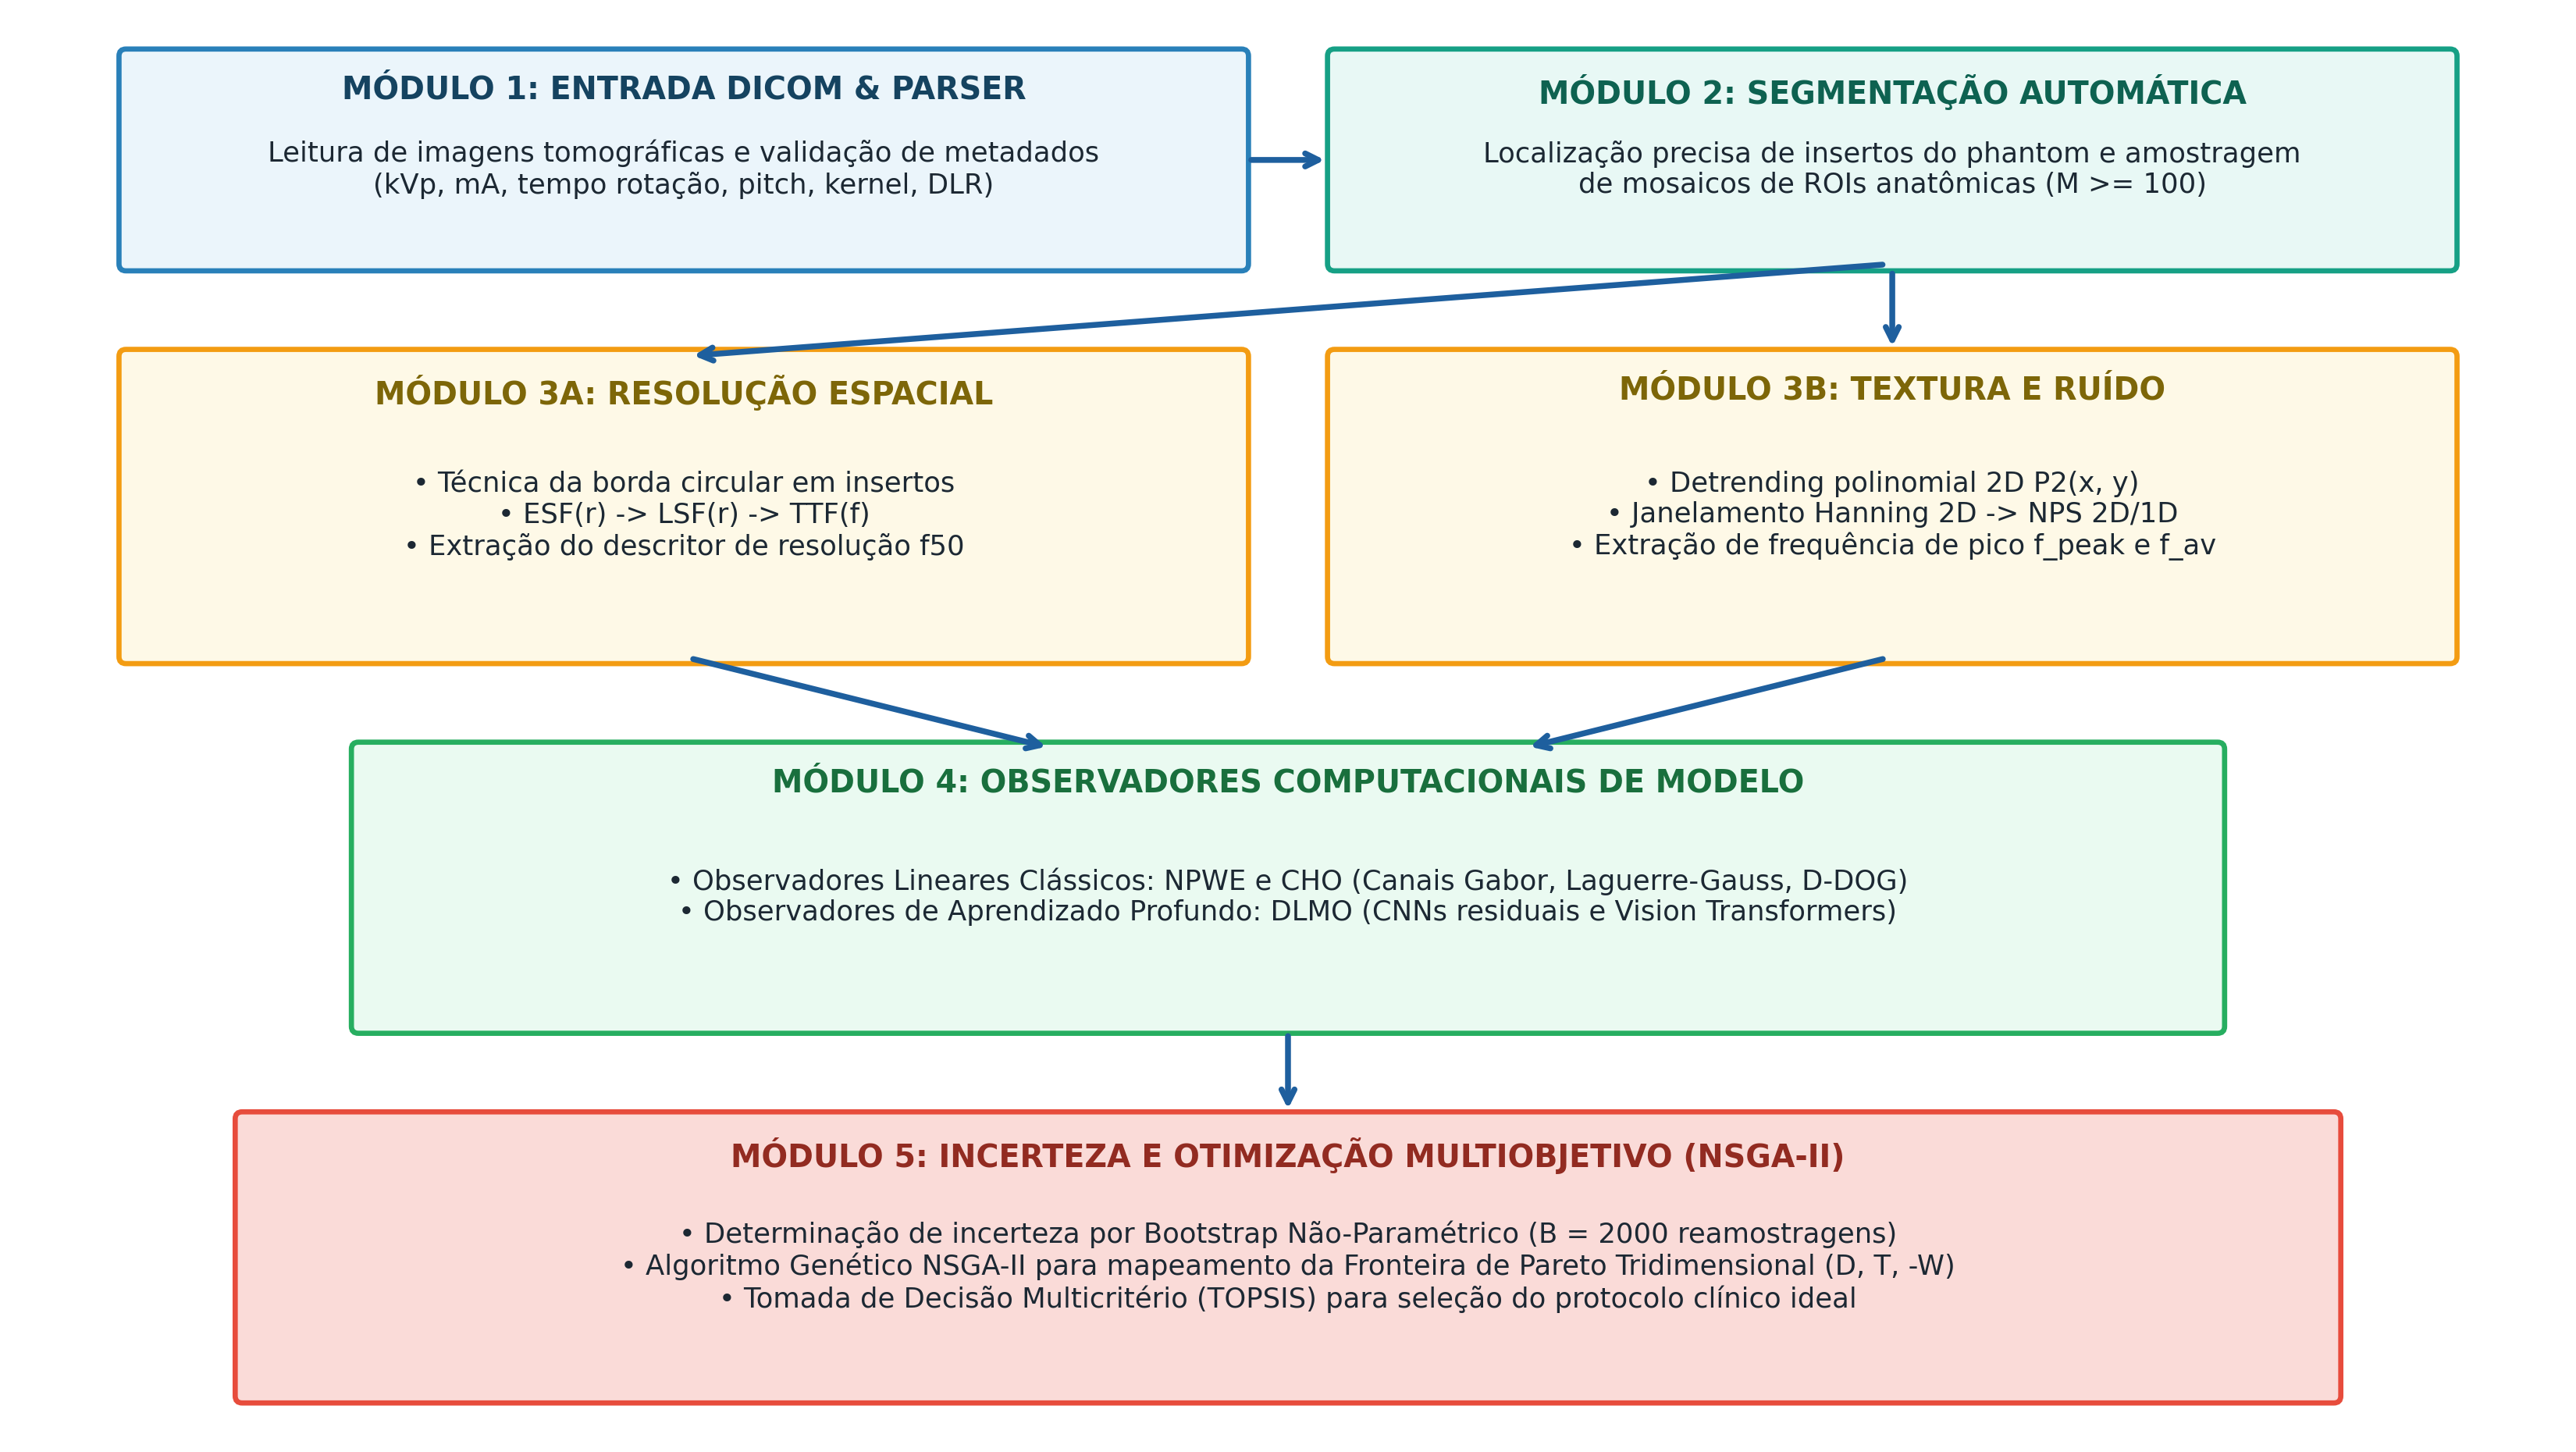
\includegraphics[width=0.95\textwidth]{figuras/flow6_software_pipeline.png}
  \caption{Arquitetura Modular do Software de Metrologia em Tomografia Computadorizada (Pipeline Integrado GDRFM-IFUSP).}
  \label{fig:software_flow}
\end{figure}

O software é composto por cinco módulos encadeados:
\begin{itemize}
  \item \textbf{Módulo 1:} Parser DICOM e validação de metadados de aquisição;
  \item \textbf{Módulo 2:} Segmentação automática dos insertos de calibração e amostragem de mosaicos com $M \ge 100$ ROIs independentes;
  \item \textbf{Módulo 3A:} Cálculo da resolução espacial da tarefa ($ESF \to LSF \to TTF \to f_{50}$);
  \item \textbf{Módulo 3B:} \emph{Detrending} polinomial 2D e cálculo do espectro de ruído ($NPS(u, v)$ e $NPS(f)$);
  \item \textbf{Módulo 4:} Cálculo da detectabilidade via observadores lineares (NPWE e CHO) e modelos por aprendizado profundo (DLMO);
  \item \textbf{Módulo 5:} Análise de incerteza por Bootstrap e otimização da Fronteira de Pareto 3D via algoritmo NSGA-II e método TOPSIS.
\end{itemize}

\section{Protocolo Metrológico Padronizado segundo o Relatório AAPM TG-233}
\label{sec:protocolo_tg233}

As aquisições tomográficas para calibração seguem as diretrizes internacionais da AAPM \cite{aapm_tg233_2019}:
\begin{itemize}
  \item Matriz de imagem de $512 \times 512$ pixels com FOV ajustado ao diâmetro do simulador ($200 \text{ a } 350 \text{ mm}$);
  \item Espessuras de corte de $0{,}5 \text{ a } 1{,}0 \text{ mm}$ para alta resolução e $2{,}5 \text{ a } 5{,}0 \text{ mm}$ para rotina clínica;
  \item Tensões de tubo de 80, 100, 120 e 140 kVp, cobrindo doses de $\text{CTDI}_{\text{vol}}$ de $0{,}5 \text{ mGy}$ a $15 \text{ mGy}$;
  \item Modelagem de lesões esféricas padronizadas com diâmetros de 3, 5, 8 e 10 mm e contrastes clínicos de $-600 \text{ HU}$ (nódulo subsólido pulmonar), $+100 \text{ HU}$ (nódulo sólido hiperatenuante) e $+30 \text{ HU}$ (lesão hepática de baixo contraste).
\end{itemize}

\section{Aspectos Bioéticos, Regulatórios e Desenho Experimental com Seres Humanos}
\label{sec:bioetica}

A condução dos testes psicofísicos 2AFC com médicos radiologistas para obtenção dos dados de calibração exige aprovação formal em Comitê de Ética em Pesquisa (CEP/CONEP):
\begin{itemize}
  \item Recrutamento de no mínimo 20 médicos radiologistas com título de especialista pelo CBR para cada anatomia clínica avaliada ($\ge 60$ leitores no total para tórax, abdome e crânio);
  \item Aplicação obrigatória de Termo de Consentimento Livre e Esclarecido (TCLE) com garantia de anonimização dos dados de desempenho individual;
  \item Monitores diagnósticos com luminância calibrada segundo o padrão DICOM GSDF ($\ge 400 \text{ cd/m}^2$) e iluminação ambiente controlada ($< 15 \text{ lux}$);
  \item Mitigação de fadiga visual através de sessões curtas com no máximo 100 a 150 pares de imagens 2AFC por sessão (duração inferior a 25 minutos).
\end{itemize}
